\section{Background: Domain-specific languages in a nutshell}
\label{sec:background}
 
We use this section to introduce some basic definitions intended to establish a unified vocabulary that facilitates the comprehension of the ideas presented in this paper. 
 
\begin{itemize}


\item{\textbf{DSLs specification $\rightarrow$}} Like general purpose languages (GPLs), DSLs are defined in terms of syntax and semantics \cite{Harel:2004b}. Hence, the specification of a DSL is a tuple $<syn,sem,M_{syn\leftarrow sem}>$ \cite{Combemale:2013}. The parameter $syn$ (the \textit{\textbf{syn}tax}) refers to the structure of the DSL and specifies each language construct in terms of its name and the relationships it has with other language constructs.

\hspace{3mm} In turn, the parameter $sem$ (the \textit{\textbf{sem}antics}) refers to the meaning of the language constructs. This meaning corresponds to the dynamic behavior that establishes the manner in which language constructs are manipulated at runtime. Finally, the parameter $M_{syn\leftarrow sem}$ refers to the mapping between the language constructs and the semantics. 

\vspace{2mm}

\item{\textbf{Technological space $\rightarrow$}} Currently, there are diverse technological spaces available for the implementation of syntax and semantics of DSLs \cite{Mernik:2005b}. Language designers can, for example, choose between context-free grammars or\\and metamodels to specify syntax. Similarly, there are at least three manners to express semantics: operationally, denotationally, and axiomatically \cite{Mosses:2001}.

\hspace{3mm} In this paper we are interested on executable DSLs (xDSLs) which syntax is specified by means of \textit{metamodels}, and semantics is specified operationally by means of \textit{domain-specific actions} \cite{Combemale:2013}. Each language construct is specified in a metaclass. The relationships between language constructs are specified as references between metaclasses. In turn, domain-specific actions are specified as java-like methods that are allocated in the metaclasses.

\end{itemize}

\textbf{Example: A DSL for finite state machines.}
Figure \ref{fig:k3-example} shows a example DSL for finite states machines. It contains three language constructs that are specified in metaclasses: \texttt{StateMachine}, \texttt{State}, and \texttt{Transition}. A state machine contains states and transitions. Those relationships are represented as containment references between the corresponding metaclasses. 

The code snippets at the bottom of Figure \ref{fig:k3-example} introduce the operational semantics to the DSL. In particular, the metaclass \texttt{StateMachine} is enriched with the operation \texttt{eval()} that contains a loop that sequentially invokes the \texttt{eval()} operation defined for the metaclass \texttt{State}. The metaclass \texttt{Transition} is enriched with the operation \texttt{fire()}.

\begin{figure}
\centering
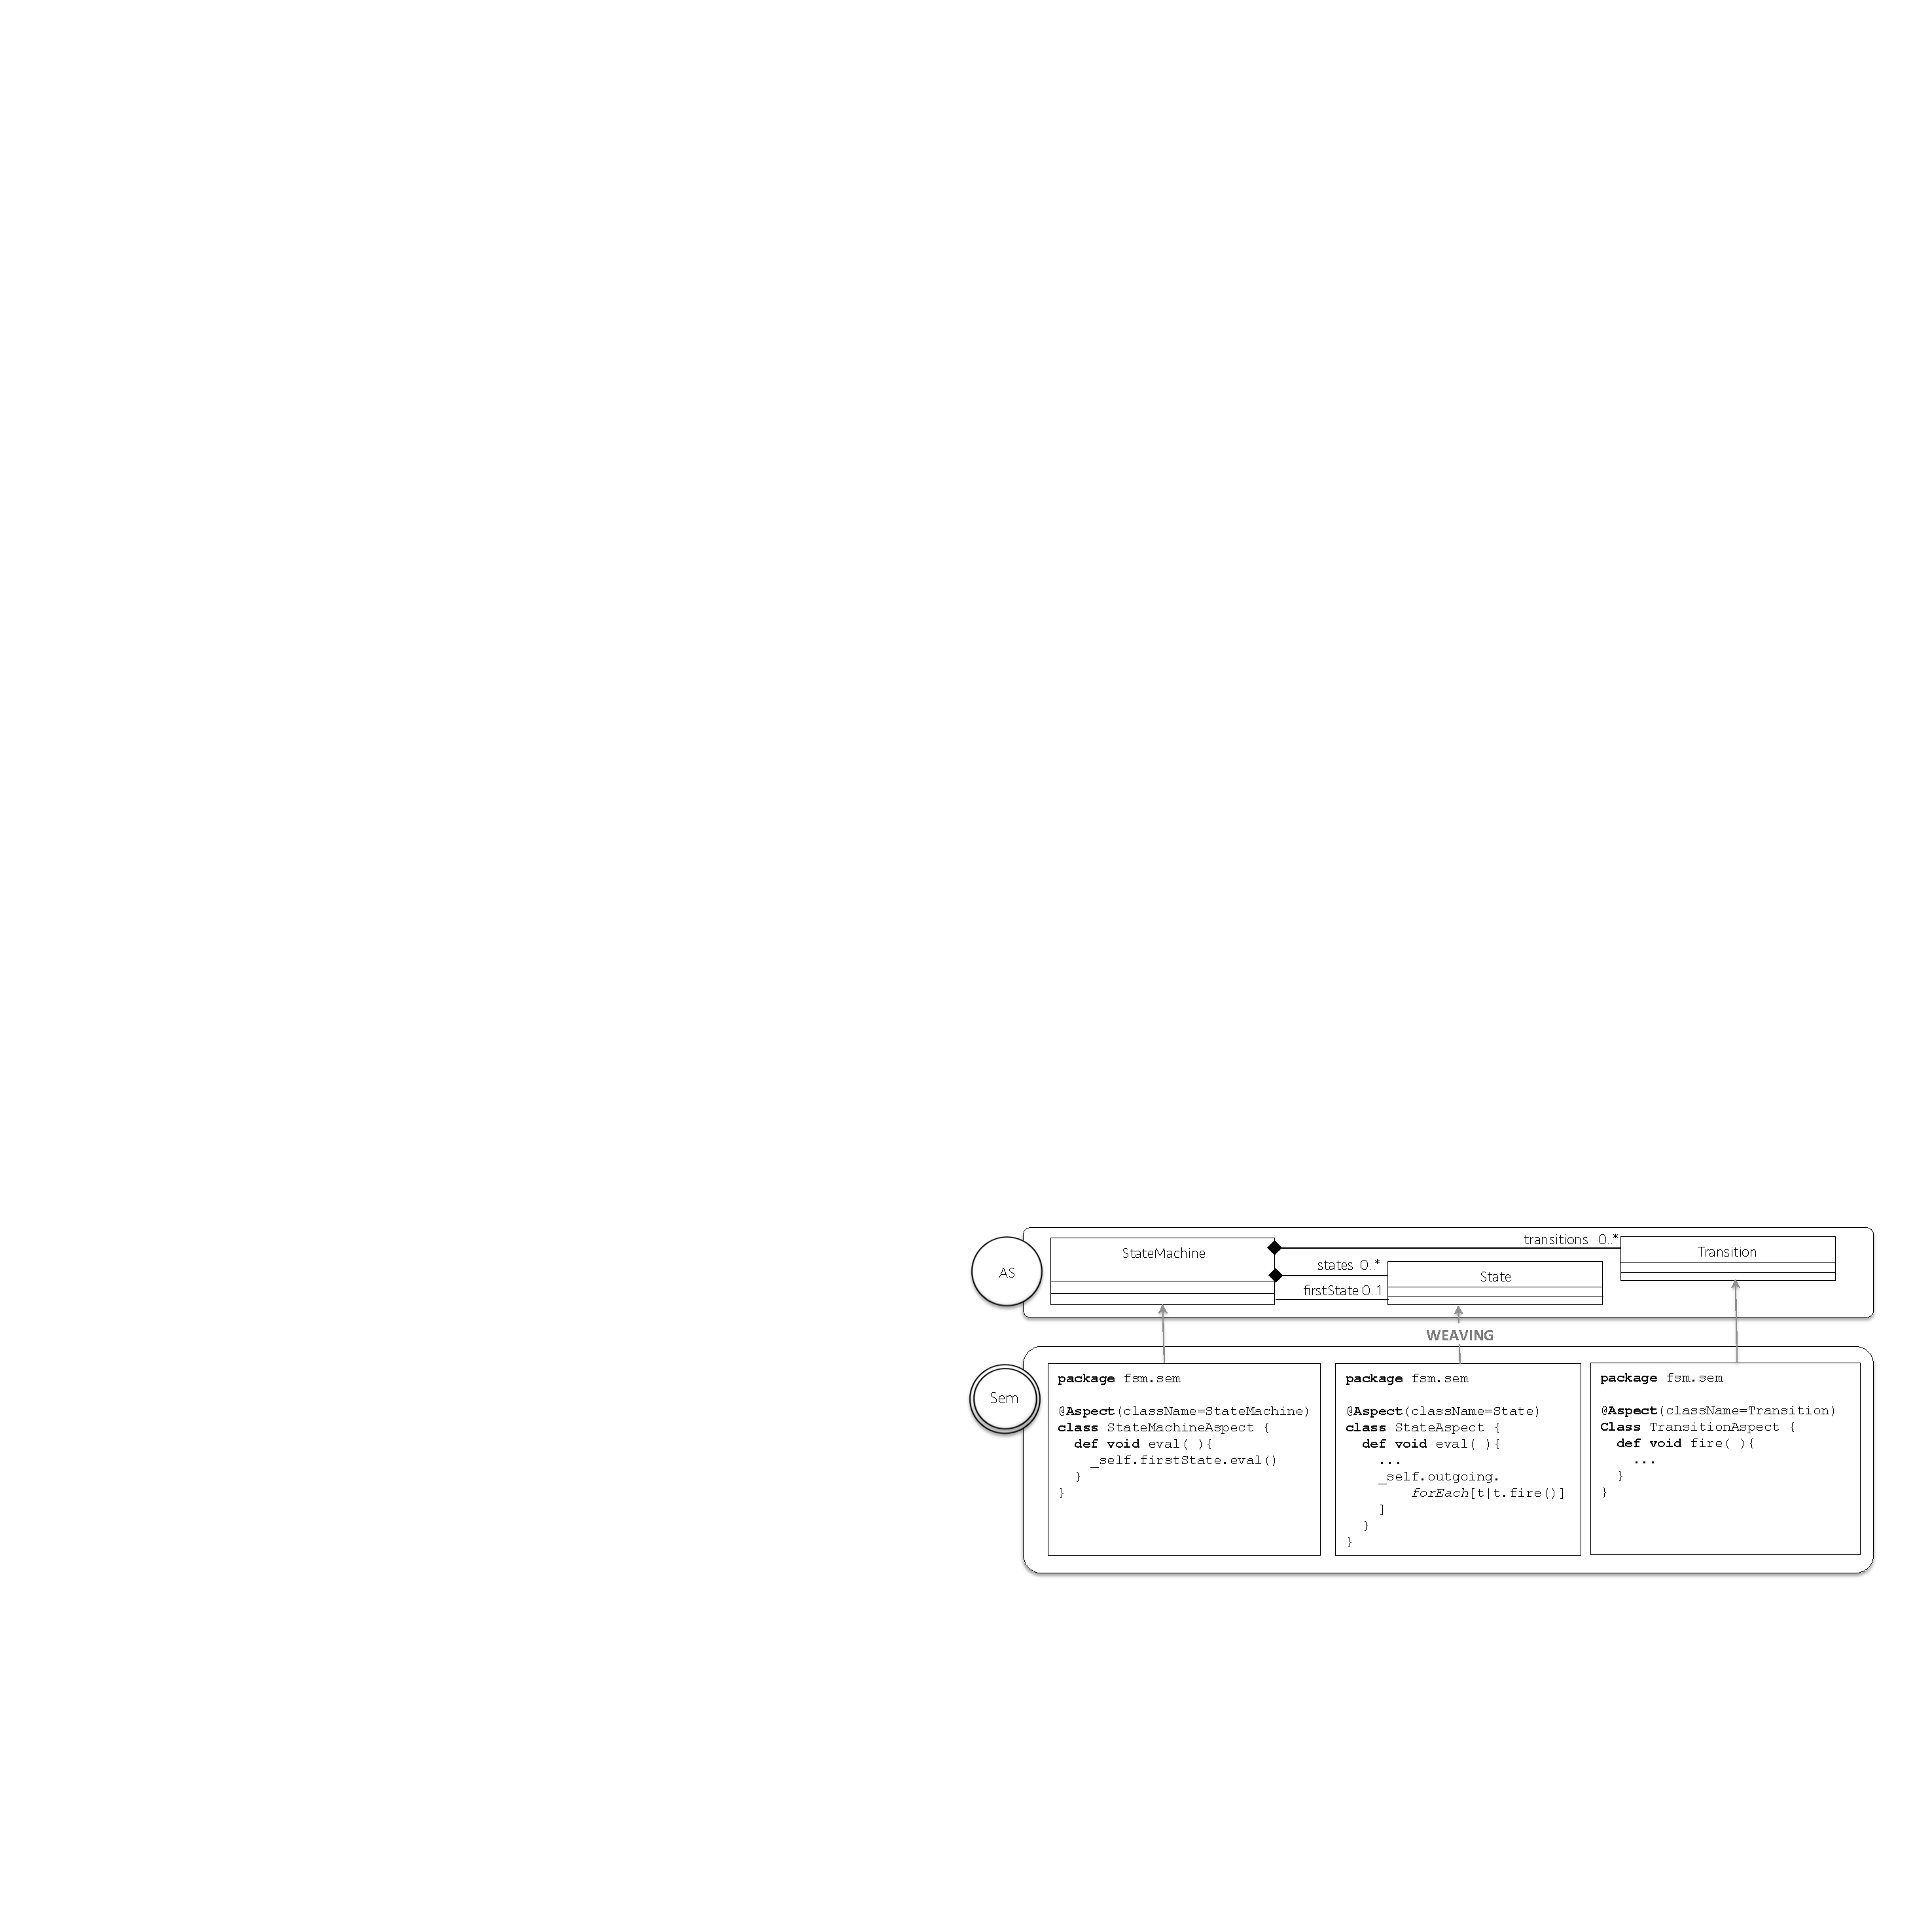
\includegraphics[width=1\linewidth]{images/k3-example-fig}
\caption{A simple DSL for finite state machines}
\label{fig:k3-example}
\end{figure}

%\todo[inline]{Este ejemplo debe ser algo que despues podamos usar para ejemplificar el funcionamiento del approach. Quizas, podamos mezclar esta sección con el motivating scenario y ahorrarnos una figura. Pero el ejemplo hay que usarlo para ejemplificar tu solucion, no solo para saber que es un xdsl.}
%As said above, we use Melange to integrate and execute the definitions of the abstract syntax and semantics of a DSL. Melange is a language for modeling in the large that facilitates the integration of the different artifacts that compose the specification of a DSL. Listing \ref{lst:fsm} illustrates the use of Melange. At the left we have an abstract representation of a language that is composed of a metamodel and three aspects implementing the semantics. At the right of the figure we have the corresponding Melange script.
 
%\vspace{4mm}
%\begin{lstlisting}[caption=Melange script for a simple FSM language, label=lst:fsm]
%language FSM {
%    syntax "fsm.mm/models/fsm.ecore"
%    
%    with fsm.sem.StateMachineAspect
%    with fsm.sem.StateAspect
%    with fsm.sem.TransitionAspect
%}
%\end{lstlisting}

%\begin{figure}
%\centering
%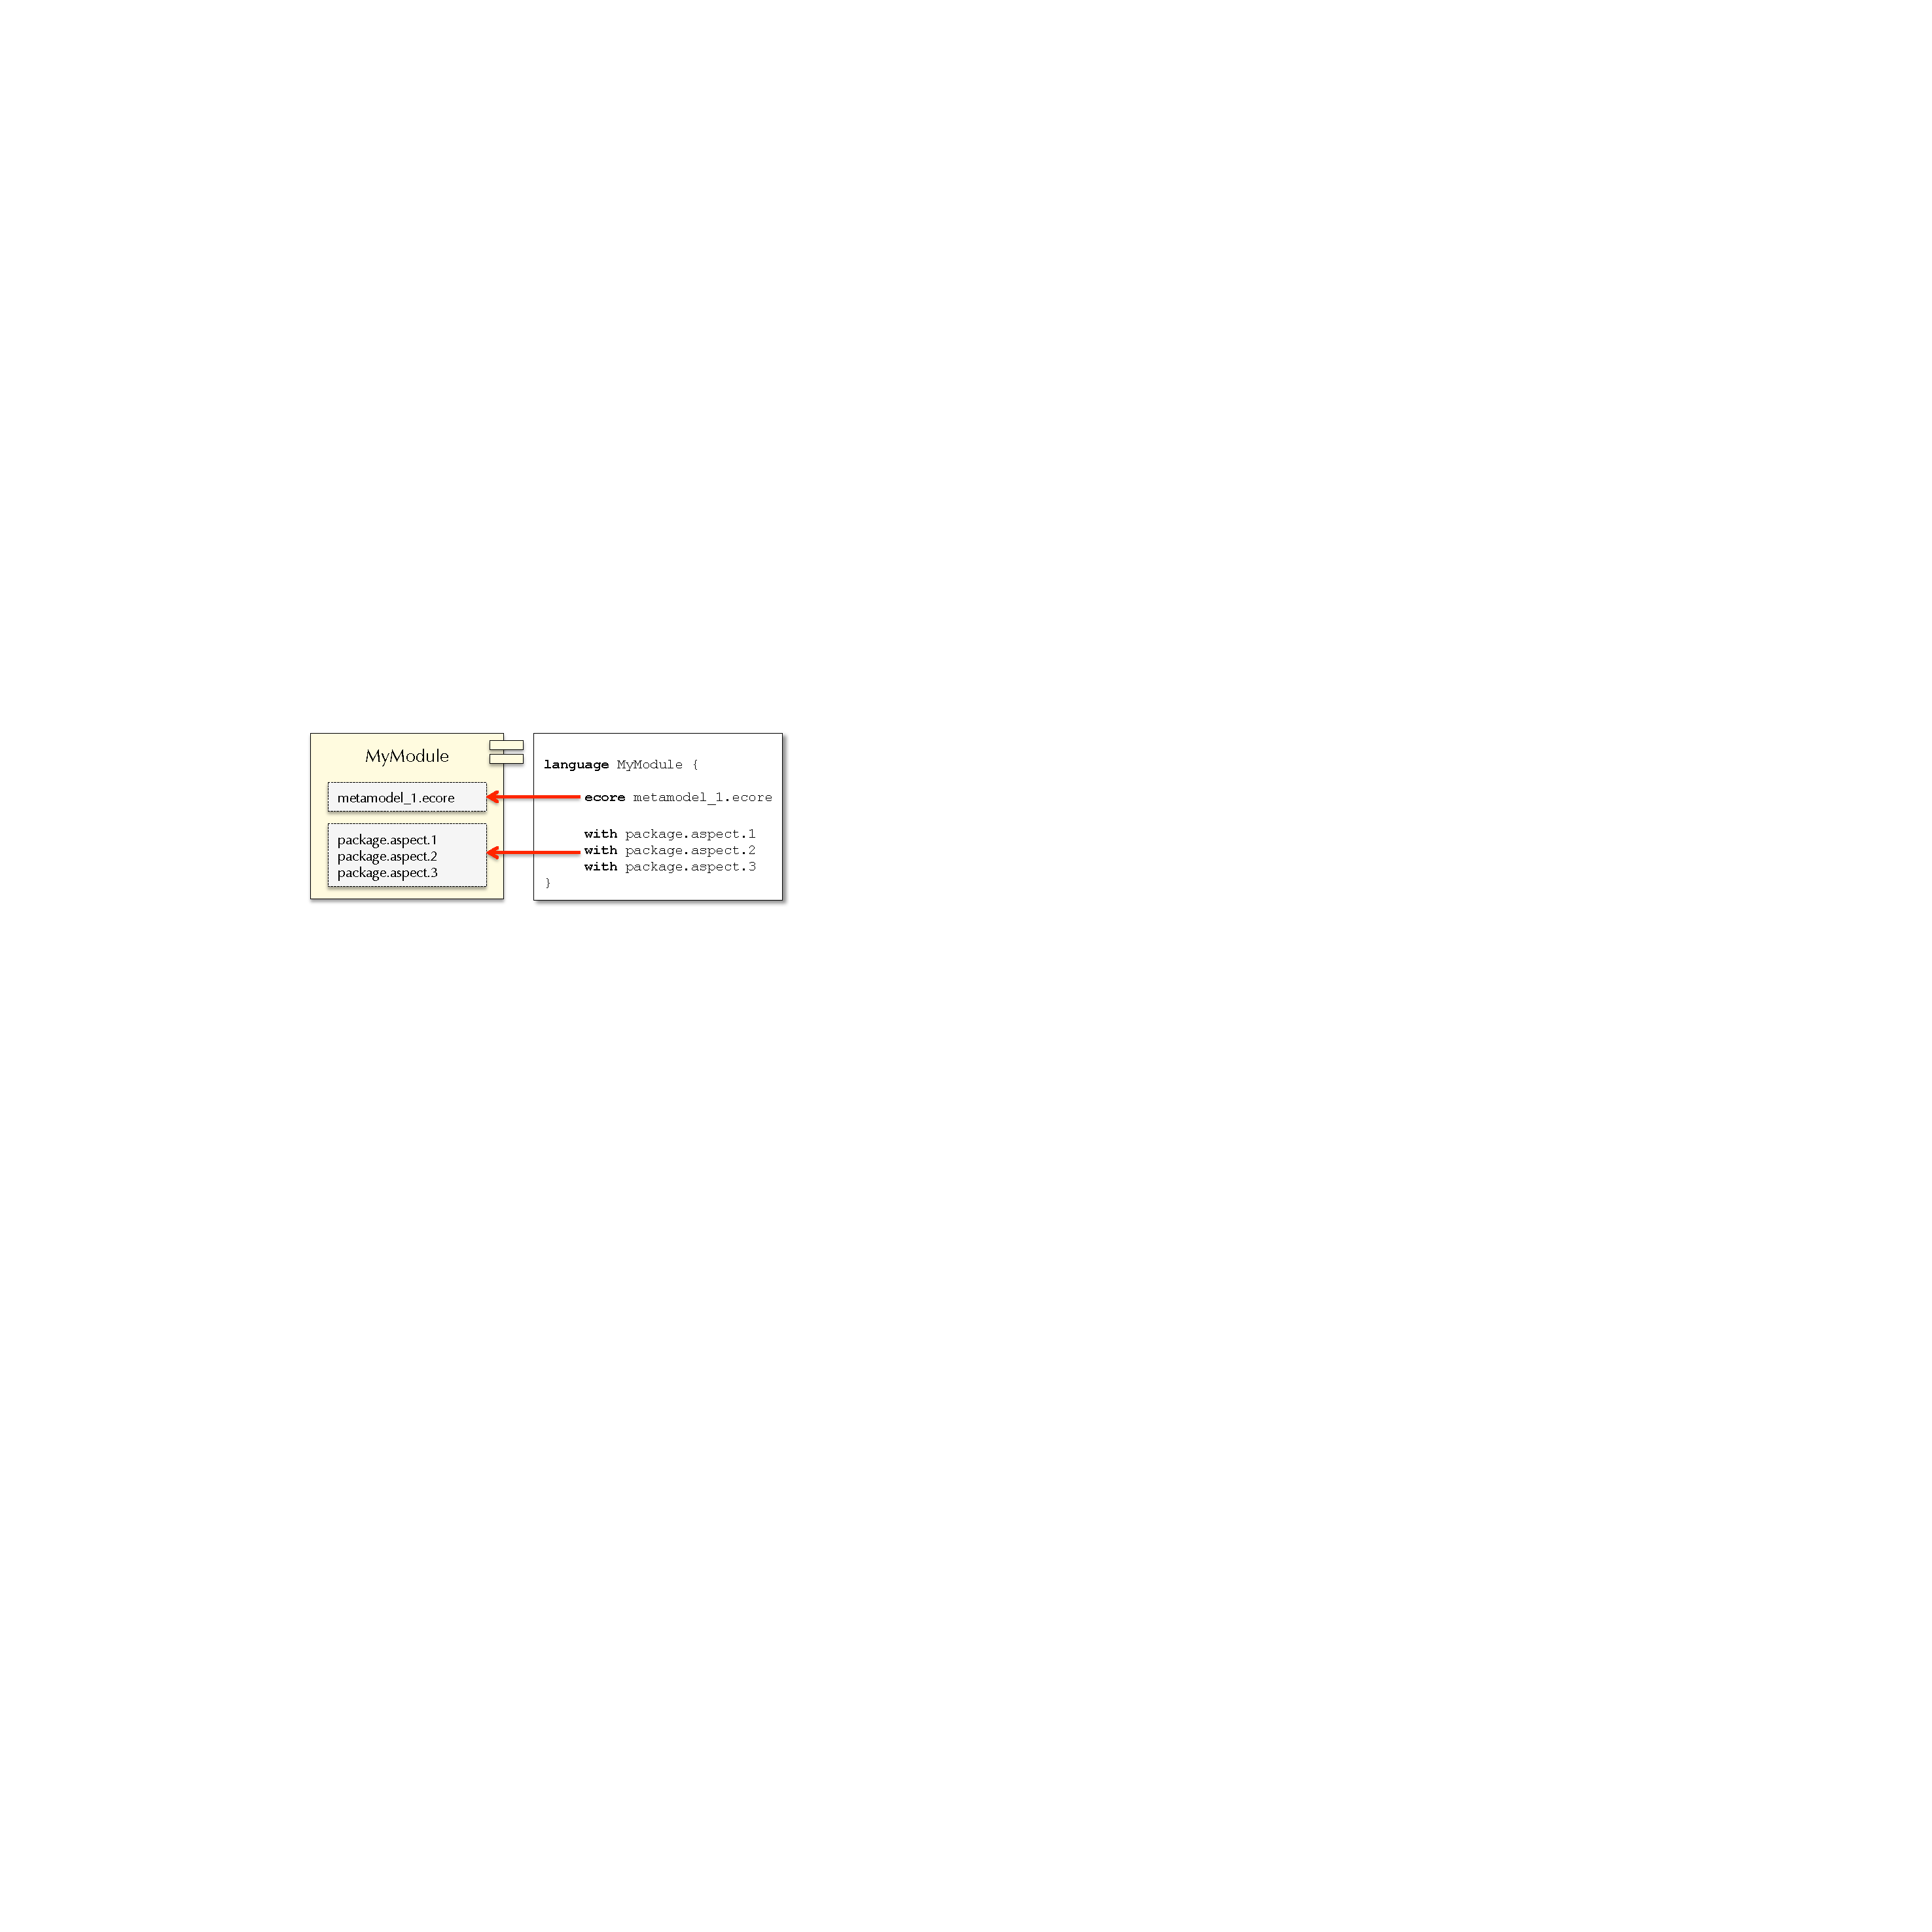
\includegraphics[width=0.8\linewidth]{images/module-melange}
%\caption{Using Melange for weaving metamodels and aspects}
%\label{fig:module-melange}
%\end{figure}
